\documentclass[12pt,a4paper]{amsart}
% ukazi za delo s slovenscino -- izberi kodiranje, ki ti ustreza
\usepackage[slovene]{babel}
\usepackage[utf8]{inputenc}
%\usepackage[T1]{fontenc}
\usepackage{amsmath,amssymb,amsfonts}
\usepackage{url}
%\usepackage[normalem]{ulem}
\usepackage[dvipsnames,usenames]{color}
\usepackage{caption}
\usepackage{lipsum}
\usepackage{tikz}
\usepackage{xcolor}

\usetikzlibrary{graphs}
\usetikzlibrary{graphs.standard}

%\makeatletter
%\renewcommand\section{\@startsection{section}{1}%
%  \z@{.5\linespacing\@plus.7\linespacing}{.5\linespacing}%
%  {\normalfont\scshape\large\centering}}
%\renewcommand\subsection{\@startsection{subsection}{2}%
%  \z@{.5\linespacing\@plus.7\linespacing}{.5\linespacing}%
%  {\normalfont\scshape}}
%\renewcommand\subsubsection{\@startsection{subsubsection}{3}%
%  \z@{.5\linespacing\@plus.7\linespacing}{-.5em}%
%  {\normalfont\itshape}}
%\makeatother

% ne spreminjaj podatkov, ki vplivajo na obliko strani
\textwidth 15cm
\textheight 24cm
\oddsidemargin.5cm
\evensidemargin.5cm
\topmargin-5mm
\addtolength{\footskip}{10pt}
\pagestyle{plain}
\overfullrule=15pt % oznaci predlogo vrstico


% ukazi za matematicna okolja
\theoremstyle{definition} % tekst napisan pokoncno
\newtheorem{definicija}{Definition}[section]
\newtheorem{primer}[definicija]{Example}
\newtheorem{opomba}[definicija]{Remark}

\renewcommand\endprimer{\hfill$\diamondsuit$}

\theoremstyle{plain} % tekst napisan posevno
\newtheorem{lema}[definicija]{Lemma}
\newtheorem{izrek}[definicija]{Theorem}
\newtheorem{trditev}[definicija]{Statement}
\newtheorem{posledica}[definicija]{Corollary}
\newtheorem{conjecture}[definicija]{Conjecture}


% za stevilske mnozice uporabi naslednje simbole
\newcommand{\R}{\mathbb R}
\newcommand{\N}{\mathbb N}
\newcommand{\Z}{\mathbb Z}
\newcommand{\C}{\mathbb C}
\newcommand{\Q}{\mathbb Q}

% ukaz za slovarsko geslo
\newlength{\odstavek}
\setlength{\odstavek}{\parindent}
\newcommand{\geslo}[2]{\textbf{#1}\hspace*{3mm}\hangindent=\parindent\hangafter=1 #2}

% naslednje ukaze ustrezno popravi
\newcommand{\program}{Financial mathematics} % ime studijskega programa: Matematika/Finančna matematika
\newcommand{\imeavtorja}{Anej Rozman, Tanja Luštrek} % ime avtorja
\newcommand{\imementorja}{Assistant Professor Janoš Vidali} % akademski naziv in ime mentorja
\newcommand{\imesomentorja}{Professor Riste Škrekovski}
\newcommand{\naslovdela}{Rich-Neighbor Edge Colorings}
\newcommand{\letnica}{2023} %letnica diplome

\begin{document}

\thispagestyle{empty}
{\large
\noindent UNIVERSITY OF LJUBLJANA\\[1mm]
FACULTY OF MATHEMATICS AND PHYSICS\\[5mm]
\program\ -- 1st cycle}
\vfill

\begin{center}{\large
\imeavtorja\\[2mm]
{\bf \naslovdela}\\[10mm]
Term Paper in Finance Lab\\[2mm]
Short Presentation\\[1cm]
Advisers: \imementorja, \\ \imesomentorja\\[2mm]}
\end{center}
\vfill

{\large
Ljubljana, \letnica}
\pagebreak

\section{Introduction}

In this paper we set out to analyse an open conjecture in a modern graph theory problem known as rich-neighbor edge coloring.

\begin{definicija}
    In an edge coloring, an edge $e$ is called $rich$ if all edges adjacent to $e$ have different colors. An edge coloring is 
    called a $rich\text{-}neighbor \ edge \ coloring$ if every edge is adjacent to some rich edge.
\end{definicija}

\begin{definicija}
    $X'_{rn}(G)$ denotes the smallest number of colors for which there exists a rich-neighbor edge coloring.
\end{definicija}

\begin{conjecture}
    For every graph $G$ of maximum degree $\Delta$, $X'_{rn}(G) \leq 2\Delta - 1$ holds.
\end{conjecture}

\begin{primer}
Let's take a look at the Petersen graph and an example of a rich-neighbor edge coloring.\\
\begin{center}
    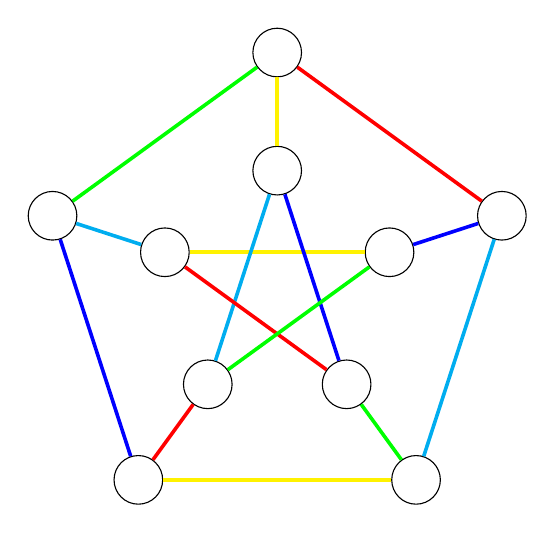
\begin{tikzpicture}[every node/.style={draw,circle, style={text opacity=0}}]
        \graph[clockwise, radius=3cm] {subgraph C_n [n=5,name=A] };
        \graph[clockwise, radius=1.5cm] {subgraph I_n [n=5,name=B] };

        % Define edge colors for the graph
        \draw[yellow, line width=1.3pt] (A 1) -- (B 1);
        \draw[blue, line width=1.3pt] (A 2) -- (B 2);
        \draw[green, line width=1.3pt] (A 3) -- (B 3);
        \draw[red, line width=1.3pt] (A 4) -- (B 4);
        \draw[cyan, line width=1.3pt] (A 5) -- (B 5);
        \draw[red, line width=1.3pt] (A 1) -- (A 2);
        \draw[cyan, line width=1.3pt] (A 2) -- (A 3);
        \draw[yellow, line width=1.3pt] (A 3) -- (A 4);
        \draw[blue, line width=1.3pt] (A 4) -- (A 5);
        \draw[green, line width=1.3pt] (A 5) -- (A 1);
        \draw[yellow, line width=1.3pt] (B 5) -- (B 2);
        \draw[cyan, line width=1.3pt] (B 4) -- (B 1);
        \draw[blue, line width=1.3pt] (B 3) -- (B 1);
        \draw[red, line width=1.3pt] (B 5) -- (B 3);
        \draw[green, line width=1.3pt] (B 4) -- (B 2);
    \end{tikzpicture}\\
\end{center}
We can see that for the Petersen graph (which is 3-regular) $X'_{rn}\leq 5$.
\end{primer}\\
\textcolor{white}{i\\ i\\ i\\ i\\ i\\ i\\ i\\ i\\ i\\ i\\ i\\ i\\ i\\ i\\}
\pagebreak

\section{Plan}

Our plan is to create an integer program that ``proves'' the conjecture for (small) regular graphs of degree 4 $\geq$ (it finds a rich-neighbor edge coloring for every $k$-regular graph on $n$ verticies) and to make a random search algorythm for checking classes of graphs that are too large to be checked individually.

\subsection{Integer Programming}

Using SageMath we plan to create an integer programming model, that checks all smaller graphs for a rich-neighbor edge coloring with $\leq 2 \Delta - 1$ colors. Our interger program looks like this:\\

minimize $t$ \hfill \textcolor{gray}{we minimize the number of colors we need}\\

subject to $\forall e: \quad \sum_{i=1}^{k} x_{ei} = 1$ \hfill \textcolor{gray}{each edge is exactly one color}\\

\ \ \ \ \ \ \ \ \ \ \ \ \ \ $\forall i \ \forall u \ \forall v, w \sim u, v \neq u: \quad x_{uv, i} + x_{uw, i} \leq 1$\\[0.1mm]
\textcolor{white}{hihi} \hfill \textcolor{gray}{edges with the same vertex are a different color}\\

\ \ \ \ \ \ \ \ \ \ \ \ \ \ $\forall e \ \forall i: \quad x_{ei} \cdot i \leq t$ \hfill \textcolor{gray}{we use less or equal to $t$ colors}\\

\ \ \ \ \ \ \ \ \ \ \ \ \ \ $\forall i \ \forall uv \ \forall w \sim u, w \neq v \ \forall z \sim v, z \neq u, w: \quad x_{uw, i} + x_{vz, i} + y_{uv} \leq 2$ \hfill \\[0.1mm]
\textcolor{white}{hihi} \hfill \textcolor{gray}{$uv$ is a rich edge $\Leftrightarrow$ all adjacent edges are a different color}\\

\ \ \ \ \ \ \ \ \ \ \ \ \ \ $\forall e: \quad \sum_{f \sim e}y_f \geq 1$ \hfill \textcolor{gray}{every edge is adjacent to some rich edge}\\

\ \ \ \ \ \ \ \ \ \ \ \ \ \ $\forall e: \quad 0 \leq y_{e} \leq 1$, $y_{e} \in \Z$\\

\ \ \ \ \ \ \ \ \ \ \ \ \ \ $\forall e \ \forall i: \quad 0 \leq x_{ei} \leq 1$, $x_{ei} \in \Z$,\\

where
\begin{align*}        x_{ei} = \begin{cases}
            1, \  \text{if edge $e$ has color $i$} \\
            0, \  \text{otherwise}
    \end{cases} & \text{and} & 
    y_{e} = \begin{cases}
        1, \  \text{if edge $e$ is rich} \\
        0, \  \text{otherwise.}
    \end{cases}
\end{align*}

 We will determine at what point the computation of rich-neighbor edge coloring becomes 
 too intense for this technique and we will then use the random search algorythm.

\subsection{Random Search}

We will construct a random search algorythm that will check if the conjecture holds for
a class of graphs that are too large to be checked individually. We plan to iterate over 
all $k$-regular graphs on $n$-vertices and based on the generated sample of 
$$
X \sim \begin{pmatrix}
    0 & 1 \\
    1 - p & p
\end{pmatrix}
$$
for a small $p$ we will check the graph or not. Since the conjecture should hold for all
graphs, we will determine the value $p$ so that we check approximately the same number of graphs for
each $k$ and $n$.

\end{document}